\documentclass{beamer}

\usetheme{MagdeburgFIN}
\usefonttheme{structurebold}
\usepackage{graphicx}
\usepackage{float}
\usepackage{url}
\usepackage{pdfpages}
\usepackage[ngerman]{babel}
\usepackage[utf8]{inputenc}


\title{Softwareprojekt - Abschlusspräsentation}
\author{Gina Seckendorf, Alexandra Koch, Jonathan Kloss}
\date{24. Januar 2017}


\begin{document}

\begin{frame}[plain]
 \titlepage
\end{frame}


\section[Agenda]{}
\begin{frame}
\frametitle{Inhalt}
\tableofcontents
\end{frame}


\section{Idee}

	\subsection{Werwölfe von Düsterwald}
\begin{frame}
\frametitle{Ablaufdiagramm - Kartenspiel}

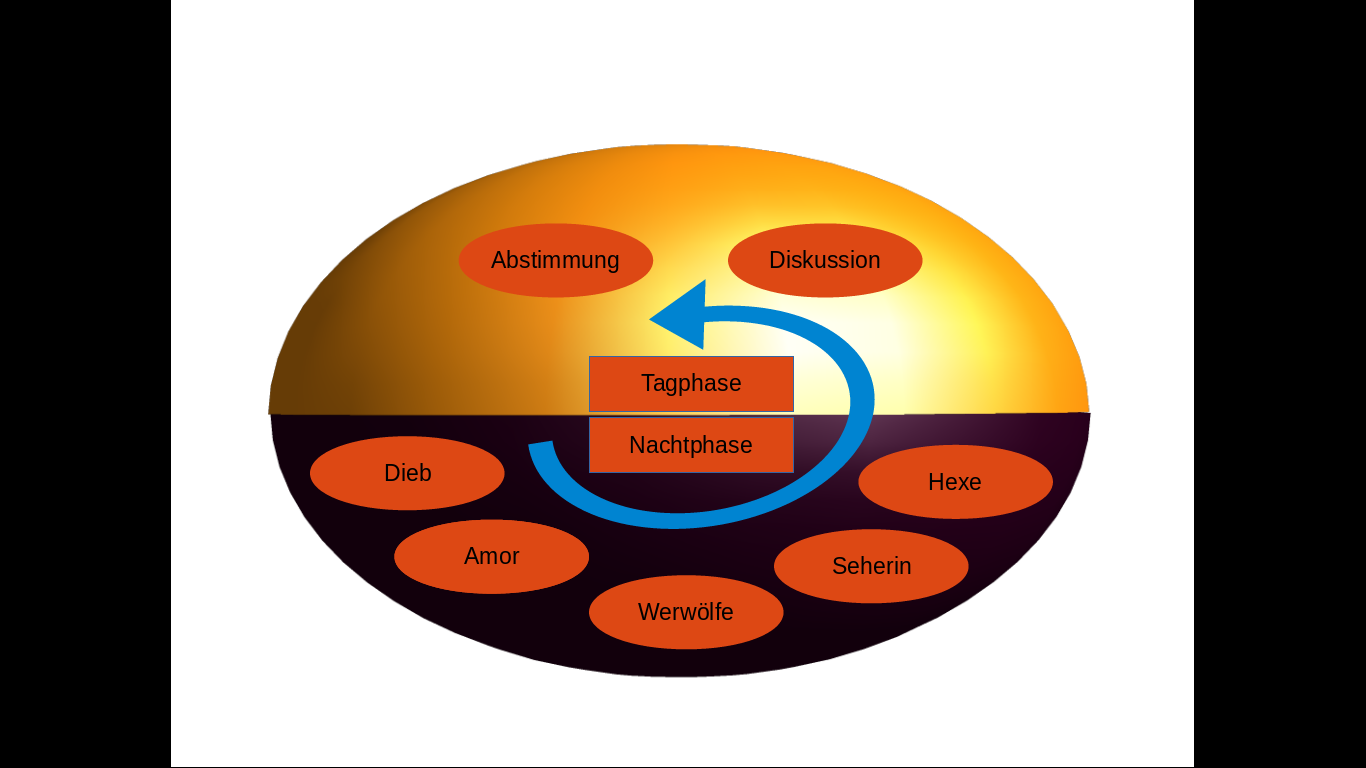
\includegraphics[width=10cm]{img/ablauf.png}
\end{frame}

\note{
	- Ablauf des Spiels erläutern\\
	- Rollenkarten verdeckt ausgeteilt/zugewiesen\\
	- getrennt in Tag- und Nachtphase\\
	- Spiel beginnt mit Nacht (alle Augen zu)\\
	- nacheinander erwachen: Dieb und Amor (nur 1x), Werwölfe, Seherin, Hexe\\
	- am Tag öffen alle die Augen und hängen einen Spieler
}

	\subsection{Mehrwert}
\begin{frame}
\frametitle{Mehrwert}
\begin{itemize}
\item Kein Spielleiter erforderlich!
\item Intuitive Bedienung
\item Einsteiger-freundlich
\item Es wird kein Kartenspiel benötigt
\item App enthält detaillierte Regelbeschreibungen %sonst muss man immer so 'unauffällig' nachfragen
\item Automatische Regelbefolgung %keine Fehler
\end{itemize}
\end{frame}


\section{Projektplanung}

	\subsection{Meilensteine}
\begin{frame}
\frametitle{Meilensteine}
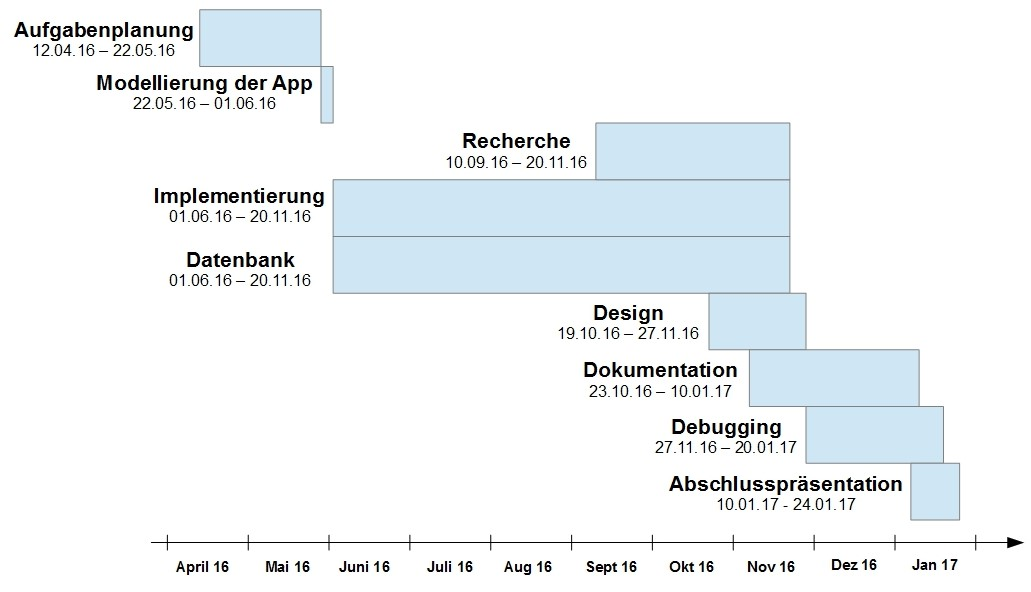
\includegraphics[width = \textwidth]{img/Meilensteine.jpg}
\end{frame}

	\subsection{Projektplan}
\begin{frame}
\frametitle{Projektplan}
\vspace{0.3 cm}
%\includegraphics[width = \textwidth]{img/projektplan.jpg}
\end{frame}

	
\section{Projektdurchführung}

	\subsection{Soll-Ist-Diagramm}
\begin{frame}
\frametitle{Soll-Ist-Diagramm}

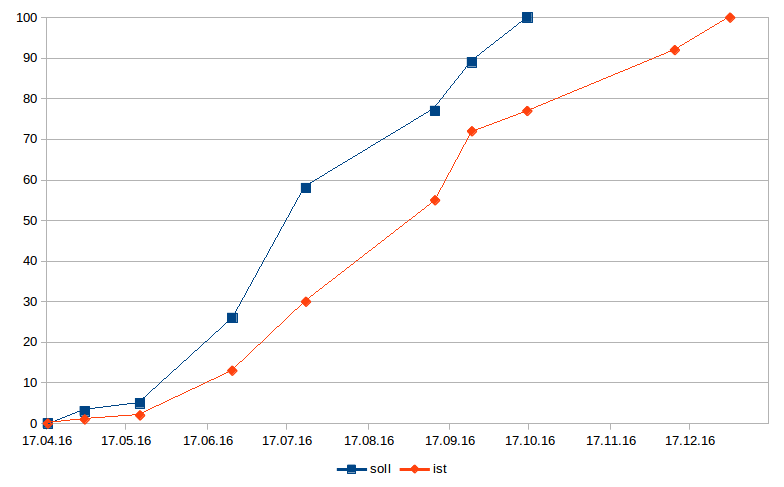
\includegraphics[width = \textwidth]{img/soll_ist_diagramm.png}

\end{frame}

\begin{frame}
\frametitle{Soll-Ist-Diagramm}

[Soll ... - Ist]

\end{frame}

\begin{frame}
\frametitle{Soll-Ist-Diagramm}

[Soll n - Ist]

\end{frame}

	
	\subsection{FINd die Werwölfe}
\begin{frame}
\frametitle{Klassendiagramm}
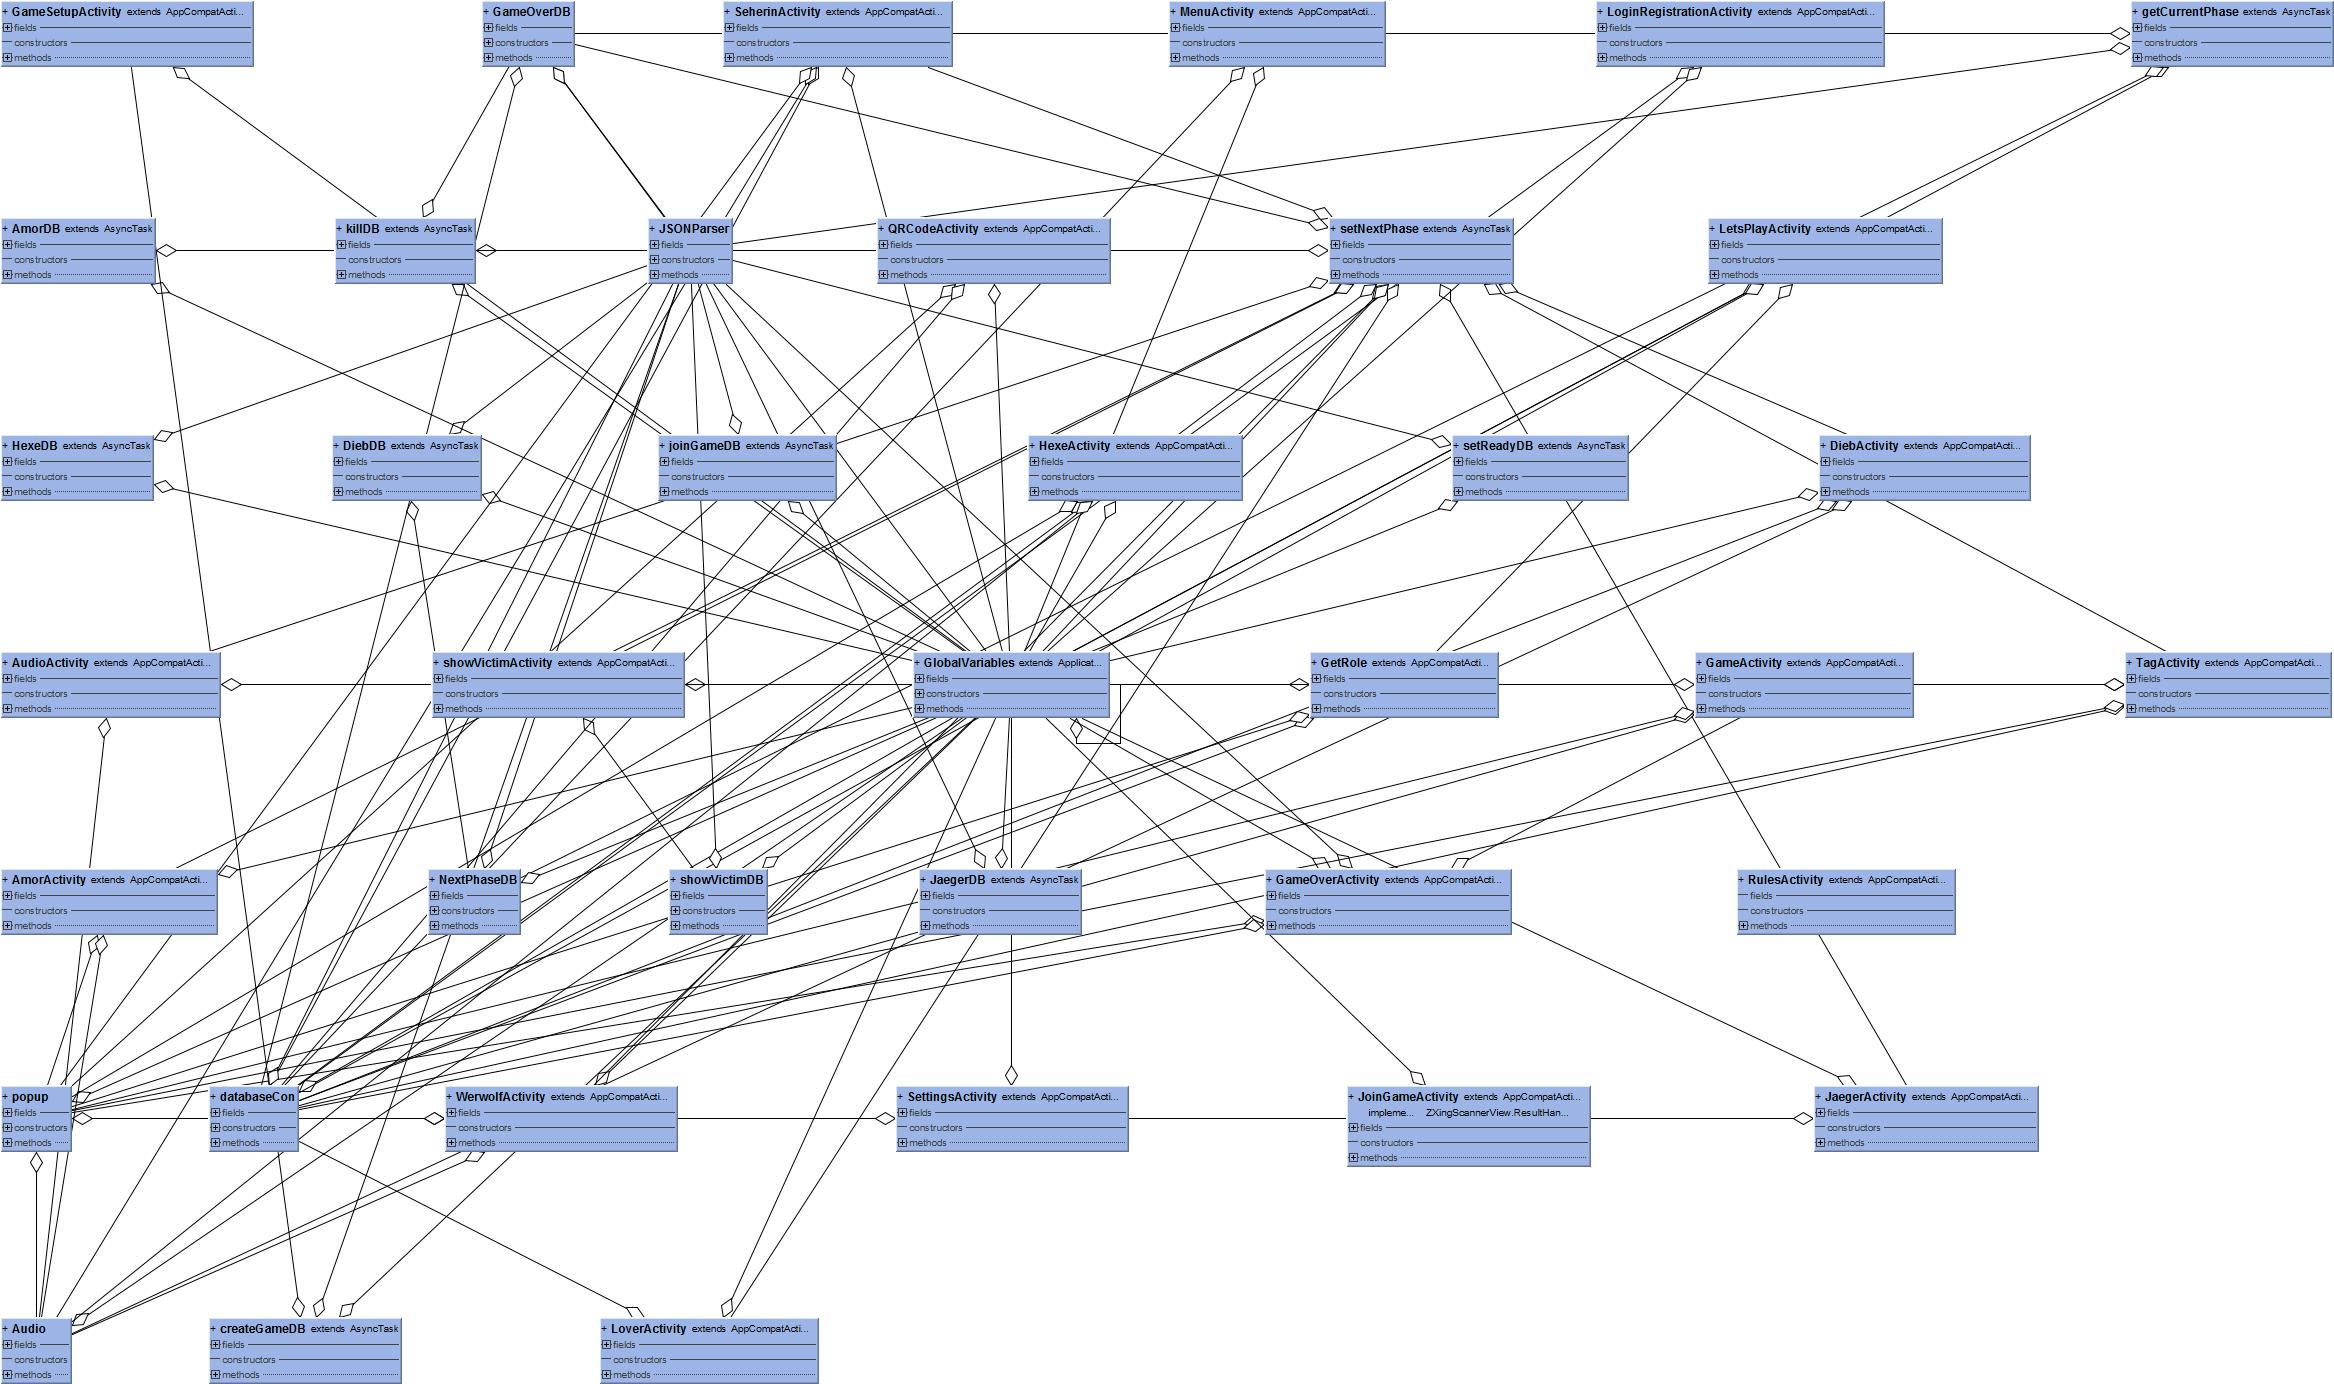
\includegraphics[width=1.0\textwidth]{img/WUML.jpg}
\end{frame}

\begin{frame}
\frametitle{Ablauf}
Screenshots; Erklärung ...
\end{frame}


\section{Projektbewertung}


	\subsection{Probleme}
\begin{frame}
\frametitle{Probleme}
\begin{itemize}
\item Umfang des Projektes einschätzen (sowohl Zeit- als auch Arbeitsumfang)
\\ $\rightarrow$ Einteilung der Arbeit
\pause
\item Kommunikation innerhalb des Teams
\pause
\item Einarbeitungszeit
\pause
\item Einteilung der Arbeit
\pause
\item Mangelnde Android-/PHP-Kenntnisse
\end{itemize}
\end{frame}
	
	
	\subsection{Was haben wir gelernt?}
\begin{frame}
\frametitle{Lessons Learned}
\begin{itemize}
\item Projektplanung
\begin{itemize}
	\item ausführliche Vorbereitung
	\item Aufgabenverteilung
	\item Zeiteinteilung
\end{itemize}
\pause
\item Struktur eines Projekts
\pause
\item Absprache untereinander
\pause
\item Teamorganisation
\pause
\item Android-spezifische Kenntnisse
\end{itemize}
\end{frame}


\begin{frame}
 \centering \textbf{Vielen Dank für Ihre Aufmerksamkeit!}
\end{frame}

\begin{frame}
\begin{center}


 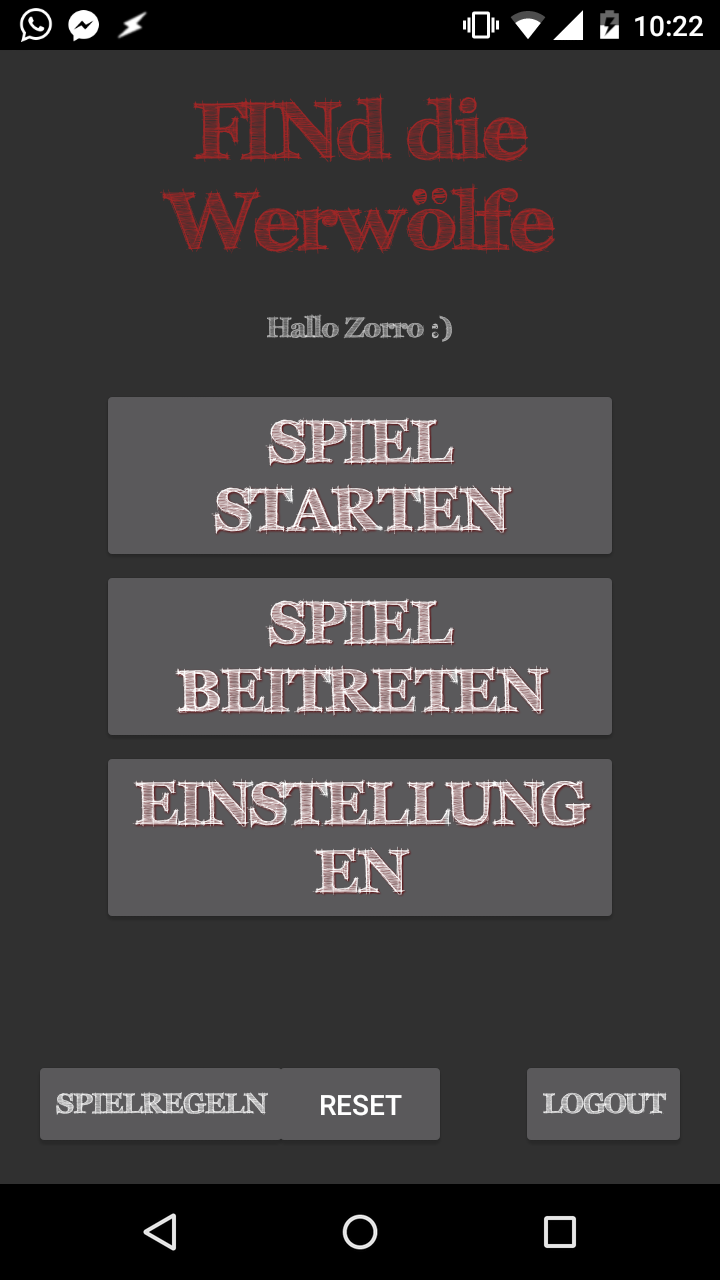
\includegraphics[width=4.1cm]{img/screenshot_menu.png}
 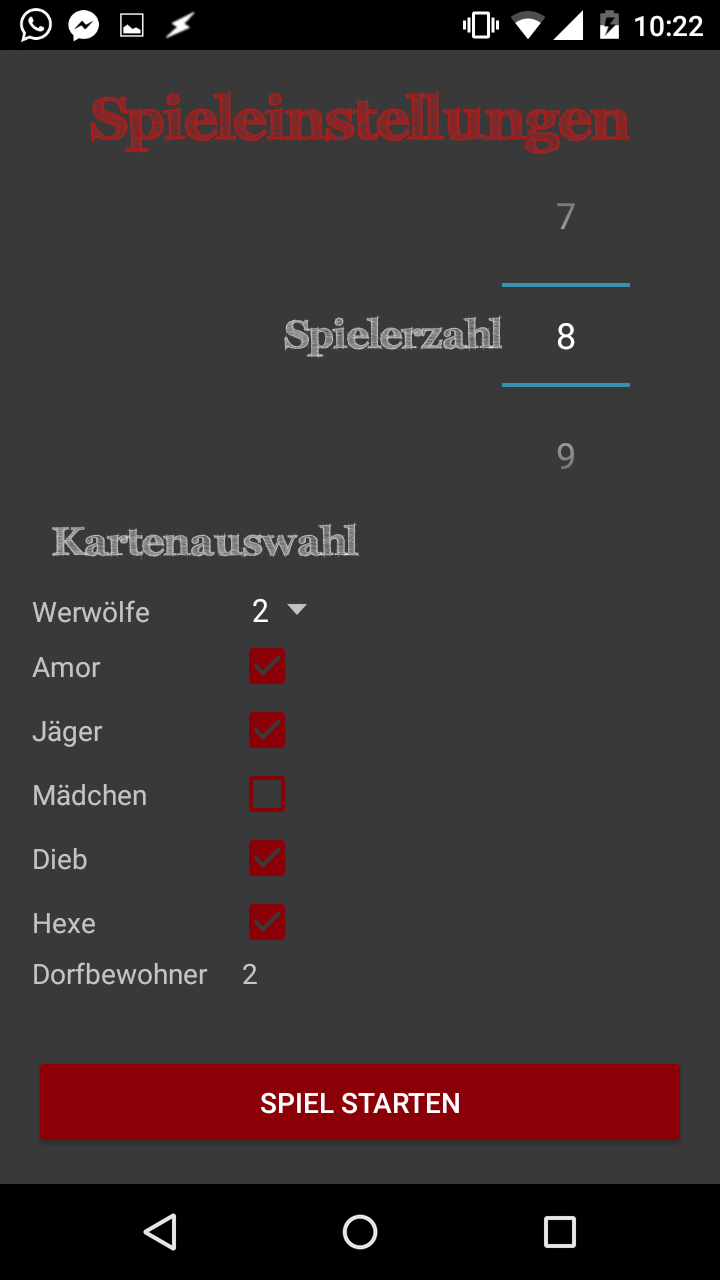
\includegraphics[width=4.1cm]{img/screenshot_create_game.png}
 \end{center}
\end{frame}


\end{document}
